\documentclass[11pt,a4paper,openright]{memoir}

% font encoding
\usepackage[T1]{fontenc}

% being able to quote
\usepackage[threshold=1]{csquotes}

% being able to use images
\usepackage{graphicx}

% columns hyphenation spacing
\usepackage{soul}
\usepackage{multicol}
\usepackage[document]{ragged2e}

% bibtex
\usepackage[backend=bibtex,bibencoding=ascii]{biblatex}
\usepackage{url}

% tables and NLP
\usepackage{tikz}
\usepackage{tikz-qtree}
\usepackage{tikz-dependency}

% graphs
\usepackage{pgfplots}
\pgfplotsset{compat=1.12}

% use xml
\usepackage{listings}

% This one includes babel in Australian mode
\usepackage{unswcover} 

% Include bibliography
\addbibresource{thesis.bib} 

% TOC configuration
\setcounter{tocdepth}{4}
\setcounter{secnumdepth}{4}
\setsecnumdepth{subsection}

\newcommand{\theTitle}{Knowledge graph construction for research literatures}
\newcommand{\theAuthor}{Alisson Oldoni}
\newcommand{\theKeywords}{natural language processing, information extraction, named entity recognition, relationship extraction}

%unicode package
\usepackage[unicode]{hyperref}
\hypersetup{colorlinks=true, linkcolor=black, citecolor=black, urlcolor=blue, pdftitle={\theTitle}, pdfauthor={\theAuthor}, pdfkeywords={\theKeywords}}

\unswschool{School of Computer Science and Engineering\\}
%% PhD is the default
\unswdegree{Master of Computing and Information Technology}

\title{\theTitle}
\author{\theAuthor}
\newsavebox{\compiledate}
\savebox{\compiledate}{\begin{otherlanguage}{australian}\today\end{otherlanguage}}
%\date{\today (document compilation)}
%% By forcing the date as follows, we let Babel do its job of formatting it
%% properly
\renewcommand\day{01}
\renewcommand\month{11}
\renewcommand\year{2016}

\begin{document}
\setlength\parindent{24pt}
\captionnamefont{\bfseries}

\frontmatter

%% If only the title page is desired
%\makeunswphdtitlepage
%% If all the administrative pages are needed too
\makeunswfrontmatter

\newpage
\thispagestyle{empty}
\strut
\vfill

%\chapter*{Acknowledgements}
%\pdfbookmark{Acknowledgements}{pdfmark:ack}
%Thanks to Camila Macagnan, my wife, for supporting through this whole process.
%I would like to thank my professor Dr. Wei Wang for all the help into delivering this project.

\chapter*{Abstract}
\pdfbookmark{Abstract}{pdfmark:abs}

%\cleardoublepage
\clearpage
\tableofcontents

\cleardoublepage
%\listoffigures

\mainmatter


%
%
% INTRODUCTION
%
%


\chapter{Introduction}
Information extraction (IE) is the process of obtaining in an automatic fashion facts and information from unstructured text that can be read by a machine \cite{Jurafsky:2000:SLP:555733}.

Historically, it mostly started with exercises on template filling based on raw natural text \cite{Moens:2006:IEA:1177314} as part of the Message Understanding Conferences (MUC) from the late 1980s and 1990s. As part of the MUC, competitions would take place in which a corpus would be made available of a specific domain, and different teams with different programs would try to extract the information from the natural text as to fill in the intended templates.

Note the following text from a news report regarding the result of a soccer match:

\blockquote{\enquote{\emph{Though Brazilian star Diego Tardelli's equaliser denied the Sky Blues victory at Jinan Olympic Sports Centre Stadium on Wednesday night, David Carney banked a precious away goal that will bode well for Graham Arnold's side when they host Shandong in next week's second round-of-16 leg. Sydney FC have taken a sizeable step towards a maiden Asian Champions League quarter-final berth after securing a 1-1 draw with Shandong Luneng in China.}}}

\begin{figure}[!htbp]
  \centering
  \RaggedRight
    \texttt{Team 1:\ \ \ \ \ \ \ \_\_\_\_\_\_\_\_\_\_\_\_\_\_\_\_\_\_\_\_} \\
    \texttt{Team 2:\ \ \ \ \ \ \ \_\_\_\_\_\_\_\_\_\_\_\_\_\_\_\_\_\_\_\_} \\
    \texttt{Winner:\ \ \ \ \ \ \ \_\_\_\_\_\_\_\_\_\_\_\_\_\_\_\_\_\_\_\_} \\
    \texttt{Location:\ \ \ \ \ \_\_\_\_\_\_\_\_\_\_\_\_\_\_\_\_\_\_\_\_} \\
    \texttt{Final Score:\ \ \_\_\_\_\_\_\_\_\_\_\_\_\_\_\_\_\_\_\_\_} \\
  \caption[An example of template to be filled in the sports domain.]{An example of template to be filled in the sports domain.}
  \label{fig:template_to_be_filled}
\end{figure}

An example of a task would be, to solely based on the above raw text, to fill in the template shown in Figure \ref{fig:template_to_be_filled}. The MUC competition would be based in various corpus and tasks based on varieties of news reports, such as satellite launches, plane crashes, joint ventures and other different data in these specific domains.

On the above example, one can observe that the \emph{Team 1} is \emph{Sydney FC}, \emph{Team 2} is \emph{Shandong Luneng}, there was no \emph{Winner}, and consequently the \emph{Location} and the \emph{Final Score}. It gets more interesting as you observe the same type of information being delivered by a different reported:

\blockquote{\enquote{\emph{SYDNEY FC take the advantage of an away goal in China, leaving the second leg of their Asian Champions League Round of 16 tie with a 1-1 draw with Shandong Luneng.}}}

Although roughly similar in this case, the approach to retrieve the data from Natural Language text needs to be able to generalise to the various ways a reporter might write such information. This effort becomes more complex as one moves through different domains and audiences of a text, such as: technical manuals, academic papers from different areas, legal text, contracts, financial news, biomedical, among others.

More recently, the output of such Information Extraction systems are used as to build other systems, more prominently Knowledge Graphs. A Knowledge Graph (KG), also known as the knowledge base, is a collection of the machine-readable database that contains entities, the attributes of entities and the relationships between entities \cite{google}. Information Extraction tools would harvest data form unstructured or semi-structured text and provide such databases.

Popular search engines such as Google \cite{google} and Bing \cite{bing} leverage Knowledge Graphs as to provide entity summary information and the related entities based on the query that the user is searching for. It is an essential foundation for many applications that requires machine understanding.

\begin{figure}[!htbp]
  \centering
    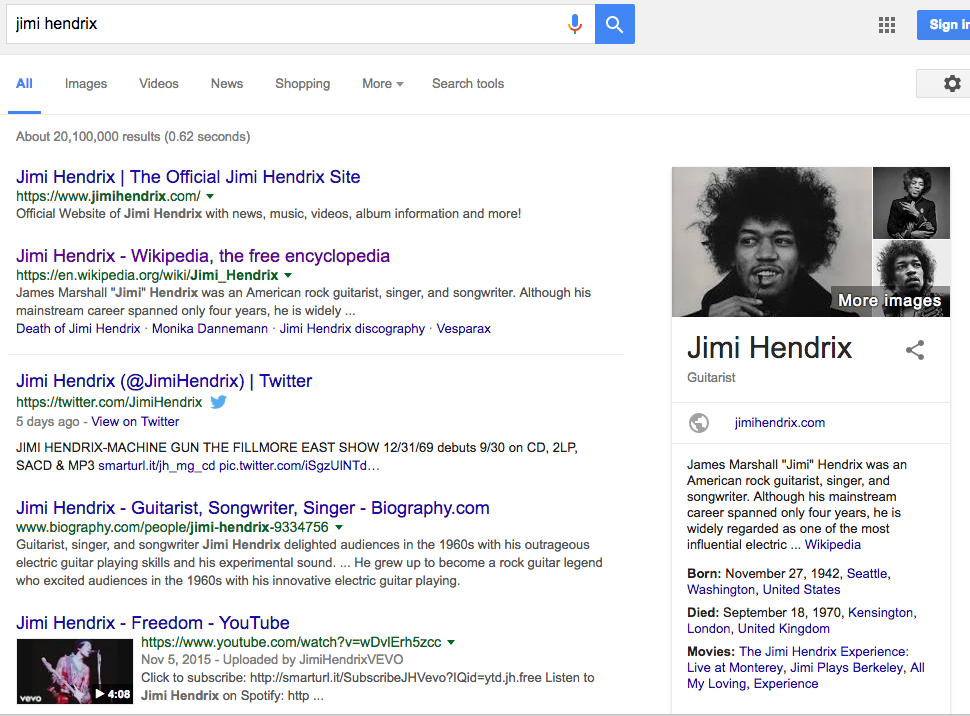
\includegraphics[width=0.8\textwidth]{./images/google_knowledge_graph}
  \caption[An example of knowledge graph application.]{An example of knowledge graph application in the Google's result page.}
  \label{fig:google_knowledge_graph}
\end{figure}

The use of Knowledge Graphs then allow users to be able to see extra information in a summarised table-like form, as to resolve their query without having to navigate to other sites. Note in the example in Figure \ref{fig:google_knowledge_graph} how the right column represents a sequence of facts of the \emph{\enquote{Jimi Hendrix}} entity, in this case an entity of the class (or type) \emph{PERSON}, such as: his official website; where and when he was born; where and when he died; and a list of movies where this person is the subject of.

Modern pipelines for building Knowledge Graphs from raw text would then encompass several Information Extraction techniques, such as the ones below:
\begin{enumerate}
  \item Discover entities in the text;
  \item Discover relationships between these entities;
  \item Perform entity disambiguation
  \item Link entities to a reference Knowledge Graph (e.g., Yago2 \cite{Suchanek2007} or DBPedia \cite{dbpedia-swj}).
  \item Improve the quality of the output via input data cleaning, robust extraction, and learning-based post-processing methods;
  \item Reason about how accurate these facts are;
  \item Finally presenting the facts in a graph (the Knowledge Graph).
\end{enumerate}

Some of these techniques will be explained further as part of this document.

In this project, we focus on studying and presenting some Information Extraction techniques as to build a domain-specific verb-centric information extraction tool that extracts relations from academic papers. More specifically, we focus on papers from the topic of databases and attempt to extract information from these papers for posterior usage by other systems with applications such as:
\begin{itemize}
	\item Allow for structured and fast search of techniques in the papers and the possible relations between them;
	\item Possibly group papers by their used techniques;
	\item Discovery of techniques to improve performance on a certain problem;
	\item Generate a hierarchy of concepts, and their use;
	\item Among others.
\end{itemize}

An existing service that organises data from academic papers is the Semantic Scholar \cite{semanticscholar} project, by Professor Oren Etzioni from Allen Institute for AI. However, Semantic Scholar only understands a limited number of relationships (such as 'cite', 'comment', 'use\_data\_set', and 'has\_caption') which are also more closely related to the meta-data about the paper, but not from the knowledge that the paper itself presents. Other similar services are Microsoft Academic Graph \cite{microsoft-academic-data}, Google Scholar \cite{google-scholar}, and CiteSeerX \cite{citeseer-x}.

\hl{In the next sections, this document will give some background information on the techniques needed to achieve the above (Chapter 2), and it will also define the problem more precisely (Chapter 3), building as to introduce the development of this research (Chapter 4). In Chapter 5 we will describe some of the results, followed by the some final remarks in Chapter 6.}


%
%
% INFORMATION EXTRACTION
%
%


\chapter{Information Extraction}

Information Extraction, a term already defined in the introduction, is a hard problem which mostly relies in attempting to use a computer to understand information explicitly stated in the form of natural language.

It is interesting to observe that, before writing down thoughts in a paper, an academic form the ideas of what facts he/she wants to express in his/hers head, and then attempt a structure to most clearly state these in text form. These multiple facts, and the relations between them, are then stated in a sentence in what is assumed to be a somewhat logical format, following the semantics of the language, whether English or any other. Following this example, one must then also assume that the future reader of this paper will use the reverse process to decode this information into facts or ideas to be understood. In fact, this assumption is what justifies the attempt of Information Extraction.

Several initiatives in the Natural Language Processing area attempt to understand and map what these semantic rules are, and how one could use a computer for tackling natural language related tasks. These initiatives are fruitful and provide advanced tools and techniques in which some will be described in this chapter.


%
%
% NATURAL LANGUAGE PROCESSING
%
%


\section{Natural Language Processing}

\emph{Natural Language Processing} (or \emph{NLP}) can be a term used to discuss any kind of computer manipulation of natural language text, also called raw text. It can mean simple things such as counting words and obtain their frequency distribution to compare different writing styles, or in a more complex sense it would require the understanding of human writings, to the extent of being able to extract information and meaning from it, or also give useful responses to them \cite{BirdKleinLoper09}. On this more complex end of the spectrum, where one wants to understand raw text, language technology and existing tools rely on formal models, or representations, of knowledge of language at the levels of morphology, syntax, semantics, among others linguistic concepts. A number of formal models including state machines, formal rule systems, logic, and probabilistic models are used to capture this knowledge from text and reason with it \cite{Jurafsky:2000:SLP:555733}.

When information is laid out in natural language form, one start the analysis of the information presented by constructing a phrase or sentence based on smaller pieces of information such as verbs, nouns, and adjectives which are called the constituents. These then build up to form sequences of simple and complex sentences.

Observing more carefully a simple sentence, such as \emph{\enquote{The police chased him.}}, it is possible to attempt to sample the different syntactic information presented in it As a first step it is possible to dissect its constituent parts as per Figure \ref{fig:pos_tags}.

\begin{figure}[!htbp]
  \centering
    \texttt{The/DT police/NN chased/VBD him/PRP ./.}
  \caption[An example of tagged sentence.]{An example of tagged sentence.}
  \label{fig:pos_tags}
\end{figure}

The first word in the sentence, \emph{The}, is a \emph{DT} or determiner. Other possible determiners include \emph{\enquote{my}}, \emph{\enquote{your}}, \emph{\enquote{his}}, \emph{\enquote{her}}. The second word is \emph{\enquote{police}} is a \emph{NN} which is the tag for a singular noun. With this information we can already tell that this sentence is speaking about something, and this something is the noun \emph{\enquote{police}}. Subsequently the tag \emph{VBD} is presented which specifically indicates the word \emph{\enquote{chased}} is a verb (an action) in the past tense. At this point one can observe that something or someone (in this case the \emph{\enquote{police}}) did something in the past.

This is already great information to have about the sentence. These tags that were added to the text in Figure \ref{fig:pos_tags} are called Part-Of-Speech tags, or POS tags \cite{Jurafsky:2000:SLP:555733}. The standardization of these tags and work to develop and tag existing text with them is done by the Penn Treebank project \cite{Marcus:1993:BLA:972470.972475}.

\begin{table}[!htbp]
  \centering
    \begin{tabular}{lll}
      \textbf{POS tag}     & \textbf{Meaning}      & \textbf{Sample} \\
      ADP  & Adpositions                           & \emph{at}, or \emph{in}        \\  
      CONJ & Coordinating conjunction              & \emph{and}, or \emph{or} \\
      DT   & Determiner                            & The                     \\
      JJ   & Adjective                             & She is \emph{tired}     \\
      JJR  & Adjective, comparative                & That one is \emph{larger} \\
      JJS  & Adjective, superlative                & That is the \emph{largest}     \\
      NN   & Noun, singular or mass                & Car                     \\
      NNS  & Noun, plural                          & Cars                    \\
      NNP  & Proper noun, singular                 & Microsoft               \\
      NNPS & Proper noun, plural                   & The \emph{Kennedys}            \\
      RB   & Adverb                                & She said \emph{firmly}         \\
      VB   & Verb, base form                       & Attack                  \\
      VBD  & Verb, past tense                      & Attacked                \\
      VBG  & Verb, gerund or present participle    & Attacking               \\
      VBN  & Verb, past participle                 & Broken                  \\
      VBP  & Verb, non-3rd person singular present & I \emph{attack}                \\
      VBZ  & Verb, 3rd person singular present     & He \emph{attacks}               
    \end{tabular}
  \caption[List of some of the possible Part-Of-Speech (POS) tags.]{List of some of the possible Part-Of-Speech (POS) tags.}
  \label{tab:pos_tags_list}
\end{table}

Note how specific the tags are, dictating the type of the word, a verb for an example, and its variation either in quantity or tense. Some other examples of these tags are shown in Table \ref{tab:pos_tags_list}. Although most of them are simple to understand, note that \emph{ADP} are the adpositions, which encompasses prepositions and postpositions. Some systems, such as the spaCy Natural Language Processing parser \cite{honnibal-johnson:2015:EMNLP, spacy} also maps these more specific tags into more general ones, for an example, while three different words in a sentence are tagged independently as \emph{VBD}, \emph{VBG} and \emph{VBZ}, they are also tagged with a \emph{VERB} tag. This is useful, if the user is not too interested in the detail of which verb variation was used.

A Part-Of-Speech Tagger is then a system that, given a raw text as input, assigns parts of speech to each word (or token) and is able to produce as output the tagged version of this text. The text in Figure \ref{fig:pos_tags} was tagged using the Stanford Log-linear Part-Of-Speech Tagger \cite{Toutanova:2003:FPT:1073445.1073478}.

\begin{table}[!htbp]
  \centering
    \begin{tabular}{llll}
      \textbf{POS Tag} & \textbf{Word} & \textbf{Prev. Word} & \textbf{Prev. Tag}  \\
      DT               & The           & <START>             & <START>             \\
      NN               & police        & The                 & DT                  \\
      VBD              & chased        & police              & NN                  \\
      PRP              & him           & chased              & VBD                 \\
      .                & .             & him                 & PRP                 \\             
    \end{tabular}
  \caption[Features for sequential POS tagging.]{Features for sequential POS tagging.}
  \label{tab:pos_tags_features}
\end{table}

The task of assigning these tags starts by deciding what are the tokens in a raw text sentence, and what are its sentences. As an example, the tokenizer needs to decide if a period symbol near a word represents an abbreviation (e.g. \emph{Dr.}) or a sentence boundary - in case of an abbreviation, this period is then considered simply a token within the sentence. Another common problem in this step is deciding if a single quote is part of a word,(e.g. \emph{\enquote{It's}}), or is delimiting a quoted part of the sentence, thus potentially hinting other semantic meanings. The Stanford POS Tagger used in this example also contain a tokenizer, which is part of the Stanford CoreNLP \cite{manning-EtAl:2014:P14-5}, a set of natural language analysis tools.

Modern POS Taggers tackle this task using a technique called Sequence Classification. A machine learning classifier model is then trained with a corpus of manually tagged text and has as an input certain features that might indicate which tag a token being currently analysed should be assigned with. Observing again the example from Figure \ref{fig:pos_tags}, but now presented in table format in \ref{tab:pos_tags_features}, it is easier to see how this learning algorithm would be trained to predict tags on unseen test. Note the second word \emph{\enquote{police}}. For this word we are providing 4 features for the learning algorithm: the manually labelled POS Tag, the word itself, the previous word and the previous POS Tag. Suppose now that this sentence in included in a bigger corpus, and this pattern is a common one and the learning algorithm is provided with a substantial amount of labelled data in which this situation repeats itself: a \emph{NN} is the second word in a sentence, with \emph{\enquote{The}} and \emph{DT} being the previous word and tag respectively.

After the training, this model would behave in a similar fashion once presented with unseen data. Suppose now the first column on Table \ref{tab:pos_tags_features} is not presented. The model would pick the first word \emph{\enquote{The}} and observe the features: \emph{<START>} and \emph{<START>} respectively and given that in our previously described corpus this is a common occurrence, it would then label this word with \emph{DT}. Now, for the second word \emph{\enquote{police}}, the features would be \emph{\enquote{The}} for previous word, and \emph{DT} for previous tag. Again, it is common for a noun to be placed after a determiner so the model assigns the label \emph{NN} to the word \emph{\enquote{police}}. The features used by the Sequence Classifies both while training and when using the model may vary and they impact the quality of the predictions it makes. The Stanford POS Tagger uses a broad use of lexical features, including jointly conditioning on multiple consecutive words \cite{Toutanova:2003:FPT:1073445.1073478}.

A helpful concept at this stage is known as the lemma. A lemma is a canonical way of representing a word which strips out variations for quantity, tense, among others \cite{Jurafsky:2000:SLP:555733}. For an example, given the words \emph{\enquote{running}} or \emph{\enquote{runs}}, NLTK \cite{BirdKleinLoper09} outputs \emph{run} as their lemma. The lemma can, for an example, be used together or instead of the existing features for training models.

\begin{figure}[!htbp]
  \centering
    \texttt{Jetstar/NNP Airways/NNPS ,/PUNC a/DET unit/NN of/ADP Qantas/NNP Airways/NNP Limited/NNP}
  \caption[An example of another tagged sentence.]{An example of another tagged sentence.}
  \label{fig:pos_tags_2}
\end{figure}

When reading a text, it is also important to understand the relation between the words or sub-sentences that are contained in the phrase, and this is specially useful for information extraction. As an example, suppose the sentence \emph{\enquote{Jetstar Airways, a unit of Qantas Airways Limited}}. There are different ways of breaking down the relationship of the words in this sentence. 

Starting again with the POS tagging discussed earlier, one can see in \ref{fig:pos_tags_2} what are the types of the words that constitutes this sentence. As a further step, it's possible to see what are the sub-sentences or parts that form the phrase structure, also called constituency parsing. The sub-sentences are connected upwards to one head (also called, \emph{parent}), and downwards to one or more governors (also called \emph{dependants}, or \emph{children}), in a recursive structure.  In Figure \ref{fig:sub_sentences_phrase_structure}, the phrase \emph{\enquote{of Qantas Airways Limited}}, which is part of the bigger phrase we are using as an example, is a prepositional phrase. A prepositional phrase lacks either a verb or a subject, and serve to assert binary relations between their heads and the constituents to which they are attached, in this case \emph{\enquote{a unit}} \cite{Jurafsky:2000:SLP:555733}. The sub-sentence \emph{\enquote{a unit of Qantas Airways Limited}} is then a noun phrase, since it contains and talks about a noun \emph{\enquote{unit}}.

\begin{figure}[!htbp]
  \centering
\Tree[.NP [.NP [.NNP \textit{Jetstar} ]
               [.NNPS \textit{Airways} ]]
          [.PUNC [., ]]
          [.NP [.NP [.DT \textit{a}    ]
                    [.NN \textit{unit} ]]
               [.PP [.IN \textit{of}    ]
                    [.NP [.NNP \textit{Qantas} ]
                         [.NNP \textit{Airways} ]
                         [.NNP \textit{Limited} ]]]]]
  \caption[A sentence and its components.]{A sentence broken down to its Phrase Structure (sub-sentences), also known as constituency parsing.}
  \label{fig:sub_sentences_phrase_structure}
\end{figure}

After discovering the structure between the phrases and its sub-phrases, finding the syntactical dependency between words themselves is also a very interesting and useful task. Continuing on the same example, one can see how the sentence states the simple fact that one company (\emph{Jetstar}) is a unit of another company (\emph{Qantas}). The dependency tree in this case tells us that \emph{Jetstar/NN} is the head of another noun \emph{Airways} and that the relation between them is of the \emph{compound} type. This relation is held between any noun that serves to modify the head noun and in this case indicate that this single entity is formed by two different words that are nouns. Note that \emph{Jetstar} has no parents and thus is the root of the sentence. The dependencies can be fully viewed is Figure \ref{fig:sub_sentences_dependency}.

The next relation is the \emph{appos} from \emph{\enquote{Airways}} to \emph{\enquote{unit}}. The appositional modifier relation indicates that the noun  immediately to the right of the first noun that serves to define or modify the meaning of the former. One now already knows that \emph{\enquote{Jetstar Airways}} is a \emph{\enquote{unit}}, and, in the business context, it probably means that it is a company that belongs to a bigger company.

\begin{figure}[!htbp]
  \centering
\begin{dependency}[theme = simple]
   \begin{deptext}[column sep=1em]
      Jetstar \& Airways \& , \& a \& unit \& of \& Qantas \& Airways \& Limited \\
   \end{deptext}
   \deproot{1}{ROOT}
   \depedge{2}{1}{compound}
   \depedge{2}{5}{appos}
   \depedge{5}{4}{det}
   \depedge{5}{6}{prep}
   \depedge[edge start x offset=+2pt]{6}{9}{pobj}
   \depedge{9}{7}{compound}
   \depedge[arc angle=50]{9}{8}{compound}
\end{dependency}
  \caption[A sentence and the dependencies between the words.]{A sentence and the dependencies between the words.}
  \label{fig:sub_sentences_dependency}
\end{figure}

Continuing the analysis, the next relation is of the \emph{prep} type and it indicates a prepositional modifier of a verb, adjective, or noun (our case), and it serves to modify the meaning of the verb, adjective, noun, or even another preposition. Note that this relation simply indicates the word pointed to by the edge is the preposition (in this case \emph{\enquote{of}}). The next relation, \emph{pobj}, indicates the actual object of the preposition and the noun phrase following the preposition and what it related to. This tree was created by the spaCy dependency parser \cite{honnibal-johnson:2015:EMNLP, spacy}. This same tree can be visualised in a more traditional tree structure in Figure \ref{fig:sub_sentences_dependency_tree}. Although not in this example, another very common relation is the relative clause modifier \emph{recmod} (or \emph{relcl} in some notations) relation. A relative clause modifier of an NP (\emph{Noun Phrase}) is a relative clause modifying the NP. The relation then in the tree points from the head noun of the NP to the head of the relative clause, normally a verb. The explanations for the cited relations in this document were obtained from the Stanford typed dependencies manual \cite{Marneffe08stanfordtyped}, and the Universal Dependencies (UD) project \cite{universal-dependencies-11234/1-1699}, both which are reference for the possible relation and contain a full lists of their meanings.

\begin{figure}[!htbp]
  \centering

\Tree[.\textit{Jetstar} \edge node[auto=right] {compound};
		[.\textit{Airways} \edge node[auto=right] {appos};
			[.\textit{unit} 
				 \edge node[auto=right] {det}; [.\textit{a} ]
				  \edge node[auto=left] {prep}; [.\textit{of}
				  	\edge node[auto=left] {pobj}; [.\textit{Limited}
				  		\edge node[auto=right] {compound}; [.\textit{Airways} ]
				  		\edge node[auto=left] {compound}; [.\textit{Qantas} ] ] ] ] ] ]

  \caption[A sentence and the dependency tree, showing the syntactical relation between these words.]{A sentence and the dependency tree, showing the syntactical relation between these words.}
  \label{fig:sub_sentences_dependency_tree}
\end{figure}

The software that is able to output a syntactical dependency tree, given a sentence, is called a dependency parser. Several different methods can be used to achieve this. One way is by defining dependency grammars, and then parsing text using these grammar. The grammar would contain words and its possible heads, and it would be applied repeatedly into the text in a process called cascaded chunking \cite{BirdKleinLoper09}. More recent methods use a process called Shift-reduce, in which the sentence is kept in a queue with the left-most token in front of the queue. The model could then decide between applying 3 operations:
\begin{enumerate}
  \item Shift: move one token from the queue to stack.
  \item Reduce left: top word on stack is head of second word.
  \item Reduce right: second word on stack is head of top word.
\end{enumerate}

A model is then trained to predict, given a text that is added to the queue, what is the next move that it should take, and what is the sequence of moves that will result in the best possible final dependency tree. This is done in a monotonic manner, in the sense that once a decision is made by the model, it cannot change it. Full working examples of this method are described in \cite{chen-manning:2014:EMNLP2014}. Other methods also use these 3 possible decisions, but allow the parser to be non-monotonic and go back in the tree and change previous decisions given new evidence form the features, such as spaCy and its dependency parser \cite{honnibal-johnson:2015:EMNLP, spacy}. Another method also uses the same set of decisions, but does a beam-search observing multiple partial hypotheses and keeping them at each step, with hypotheses only being discarded when there are several other higher-ranked hypotheses under consideration, such as the Syntaxnet parser \cite{google-syntaxnet, DBLP:journals/corr/AndorAWSPGPC16}. All these cited models use neural networks as the method to form the model.

As a further example, besides providing dependency parsing tree, spaCy also provides an iterator so you can obtain what is called the noun chunks of the document. The noun chunks are smaller pieces of the sentences within the document that are base noun phrases, or a 'NP chunk' (as per Figure \ref{fig:sub_sentences_phrase_structure}). They are noun phrases that do not permit other NPs to be nested within it – so no NP-level coordination (e.g.: \emph{\enquote{cat/NN and/CONJ dog/NN}}), no prepositional phrases, and no relative clauses \cite{spacy}.

Other problems tackled by the Natural Language Processing discipline and that are relevant for Information Extraction are \emph{Coreference resolution} and \emph{pronominal anaphora resolution}. Coreference resolution intends to define all possible entities that a text can reference to in some sort of definitive list, or more precisely a \emph{discourse model}, find in the text all the chained references to these entities, and link them to the specific entities. While very similar in nature, pronominal anaphora resolution is more simple as it is the problem of resolving in a given sentence to which previous NN (noun) or NNP (proper noun) a single PRP (pronoun) refers to \cite{Jurafsky:2000:SLP:555733}.

Take for an example the sentence \emph{\enquote{John is a quiet guy, but today he is furious.}}, the initial mention of the entity \emph{John} appears in the first token. Token five talks about a \emph{guy}, which although not a pronoun, is still a reference to the previous entity in the first word. The ninth token is a pronoun and again refers to the same \emph{John}, so is part of the chain of mentions. The full resolution chain would be denoted in Figure \ref{fig:sub_sentences_coreference}.

Normally these systems work towards analysing pairs of tokens using a probabilistic model, and then decide how likely they are references for the same entity. More recent approaches also group possible tokens in a cluster and use cluster-level features to determine the chains of coreferences \cite{clark2015entity}. The tool used to extract Figure \ref{fig:sub_sentences_coreference} is the Stanford Coreference Resolution annotator \cite{clark2015entity}, which is part of the latter group of tools that use cluster level features. This annotator is also part of the CoreNLP toolset \cite{manning-EtAl:2014:P14-5}.

\begin{figure}[!htbp]
  \centering
\begin{dependency}[theme = simple]
   \begin{deptext}[column sep=1em]
      John \& is \& a \& quiet \& guy \& , \& but \& today \& he \& is \& furious \& . \\
   \end{deptext}
   \deproot{1}{mention}
   \depedge{9}{5}{coref}
   \depedge{5}{1}{coref}
\end{dependency}
  \caption[A sentence, the mentions of an entity, and the proposed coreference resolutions.]{A sentence, the mentions of an entity, and the proposed coreference resolutions.}
  \label{fig:sub_sentences_coreference}
\end{figure}

All linguistic data mentioned in this section is data that can be obtained from the raw text itself, and is then the base for several features in which methods for Information Extraction act on.


%
%
% INFORMATION EXTRACTION
%
%


\section{Information Extraction}

The IE (Information Extraction) process is described by the following subtasks: Named Entity Recognition (NER), Coreference Resolution, Entity Disambiguation, Relation Extraction (RE), Event Detection, and Temporal Analysis \cite{Jurafsky:2000:SLP:555733}. The main subtasks relevant to this report will be described further in this section.

Once the information is extracted it is then used for tasks such as Template Filling \cite{Jurafsky:2000:SLP:555733}, Question and Answering systems \cite{Moens:2006:IEA:1177314}, or stored as a Knowledge Graph for downstream logical reasoning or for further queries.

\begin{table}[!htbp]
  \centering
  \RaggedRight
    [\textsubscript{PER} James Cook] was born on 27 October 1728 in the village of [\textsubscript{LOC} Marton] in [\textsubscript{COUNTY} Yorkshire].
  \caption[An example of NER.]{An example of Named Entity Recognition (NER).}
  \label{tab:james_cook}
\end{table}

Named Entity Recognition (NER) is the process of, given a sentence, identify and extract what are the entities that are part of it. Once the entity is detected, it needs to be classified within the classes of the given domain - in the spirit of the previous examples this would be e.g.: \emph{CITY} or \emph{PERSON}. Different types of entities are relevant to context of the data being worked with. A few approaches exist for the problem of NER, mostly related to Pattern Matching or Sequence Classification.

\begin{table}[!htbp]
  \centering
    \begin{tabular}{ll}
      \textbf{Pattern}          & \textbf{Would yield ENTITY of type} \\
      {[PERSON]} was born       & PERSON            \\
      in the village of {[LOC]} & LOCATION          \\
      in {[LOC]}                & LOCATION           
    \end{tabular}
  \caption[Patterns for NER.]{Examples of Named Entity Recognition (NER) patterns, based on the sentence from Table \ref{tab:james_cook}.}
  \label{tab:james_cook_patterns}
\end{table}

Observe, for an example, the sentence in Table \ref{tab:james_cook}. Several articles regarding prominent figures, either historical or of our current society, can be of the format \emph{\enquote{Jimi Hendrix was born}}. One approach might be Pattern Matching, which is to mine the input natural language text while looking for the pattern \emph{\enquote{[ENTITY] was born}}, using Regular Expressions (Finite-State Automata) \cite{Jurafsky:2000:SLP:555733}. The entities found by this pattern would then also receive the \emph{PERSON} class. This pattern would miss the sentence \emph{\enquote{Jimi Hendrix, born in Seattle}} since it does not fit the pattern and, because of this, one generally needs to build a list or database of patterns to work with in a corpus. An example of such database was generated by the PATTY system \cite{Nakashole:2012:PTR:2390948.2391076}. Table \ref{tab:james_cook_patterns} depicts other possible similar patterns.

Another way to extract entities from text is to frame the NER problem as a Sequence Classification problem, similar to the POS tagging problem described earlier. It requires the training of a classifier in which, given the class of the previous word, and other surrounding features of the current word, will attempt to guess if the current word is an entity, and if it is, also guesses its class.

To achieve this, previously annotated data with existing sentences and its entities is needed. This can be obtained by manually labelling data, or by semi-automated methods, like the one proposed later by this document. The format in which this annotated data is provided varies, however the IOB format (Table \ref{tab:james_cook_iob}) is more commonly used in several of the NER tools, including NLTK \cite{BirdKleinLoper09} and the popular Stanford Named Entity Recognizer (NER) \cite{Finkel:2005:INI:1219840.1219885}, part of the Stanford CoreNLP \cite{manning-EtAl:2014:P14-5}. Stanford CoreNLP provides a set of natural language analysis and information extraction tools.

\begin{table}[!htbp]
  \centering
    \begin{tabular}{ll}
      \textbf{Word}          & \textbf{Tag} \\
      James                  & B-PERSON \\
      Cook                   & I-PERSON \\
      was                    & O \\
      born                   & O \\
      on                     & O \\
      27                     & B-DATE \\
      October                & I-DATE \\
      1728                   & I-DATE \\
      in                     & O \\
      the                    & O \\
      village                & O \\
      of                     & O \\
      Marton                 & B-LOC \\
      in                     & O \\
      Yorkshire              & B-LOC \\
      .                      & O \\
    \end{tabular}
  \caption[IOB-formatted sentence.]{Example of IOB-formatted sentence used to train classifiers for the Named Entity Recognition (NER) task, based on the sentence from Table \ref{tab:james_cook}.}
  \label{tab:james_cook_iob}
\end{table}

The IOB format also helps remove ambiguity in case there are two contiguous entities of same class without any word tagged as \emph{O} in between. In practice these cases are somewhat rare in several domains, and even when trained with such tags classifiers struggle to accurately determine the boundaries of an entities, and thus a simplified version of this annotation without the \emph{B-} and \emph{I-} prefixes is more commonly used \cite{Surdeanu:2011:CIE:2021153.2021155}.

The Stanford Named Entity Recognizer (NER), also known as CRFClassifier \cite{Finkel:2005:INI:1219840.1219885}, provides a general implementation of (arbitrary order) linear chain Conditional Random Field (CRF) sequence models. A CRF is a conditional sequence model which represents the probability of a hidden state sequence given some observations.

Several relevant features can be used as an input during the training of a NER CRF classifier model. In Table \ref{tab:ner_features}, examples are presented. The Word Shape feature is an interesting addition from recent research, as it captures the notion that most entities are written in capital letters, or starting with capital letter, or containing numbers in the middle of the word, and other specific shapes.

\begin{table}[!htbp]
  \centering
    \begin{tabular}{ll}
      \textbf{Feature}          & \textbf{Description} \\
      Word                      & The current word being classified.          \\
      N-grams                   & \parbox[t]{9cm}{A feature from n-grams, i.e., sub-strings of the word.} \\
      Previous Class            & The class of the immediate previous word.          \\
      Previous Word             & The previous word.          \\
      Disjunctive               & \parbox[t]{9cm}{Disjunctions of words anywhere in the left or right.} \\
      Word Shape                & \parbox[t]{9cm}{The shape of the word being processed captured using. In general replaces numbers with \emph{d}, \emph{x} to lower-case letters, and \emph{X} to upper-case letters.} \\
    \end{tabular}
  \caption[Possible features to train the CRFClassifier.]{Examples of features used to train the CRFClassifier \cite{Finkel:2005:INI:1219840.1219885}.}
  \label{tab:ner_features}
\end{table}

In addition to the above methods another useful technique is the use of gazetteers. Gazetteers are common for geographical data, where government provided lists of names can contain millions of entries names for all manner of locations along with detailed geographical, geologic and political information \cite{Jurafsky:2000:SLP:555733}.

Relation Extraction (RE) is the ability to discern the relationships that exist among the entities detected in a text \cite{Jurafsky:2000:SLP:555733}, and is naturally the next challenge after being able to detect entities. It is generally denoted as a triplet: two entities, and the one relation between them (Table \ref{tab:relation_example}). It can be done using Pattern Matching, Classifiers, or purely by exploiting linguistic data available form a sentence. The previously described Pattern Matching technique from NER can be improved upon in the Relation Extraction step, and involve more than one entity, yielding binary relations. This approach is used in tools such as PROSPERA \cite{Nakashole:2011:SKH:1935826.1935869} or those mined by PATTY \cite{Nakashole:2012:PTR:2390948.2391076}. More specifically, examples of patterns mined by PATTY for the \emph{graduatedFrom} relation are seen in Figure \ref{fig:patty_examples}.

\begin{table}[!htbp]
  \centering
  \RaggedRight
    \texttt{Located\_In(Kiel, Germany)} \\
  \caption[An example of a triplet that represents a relation.]{An example of a triplet that represents a relation.}
  \label{tab:relation_example}
\end{table}

\begin{figure}[!htbp]
  \centering
    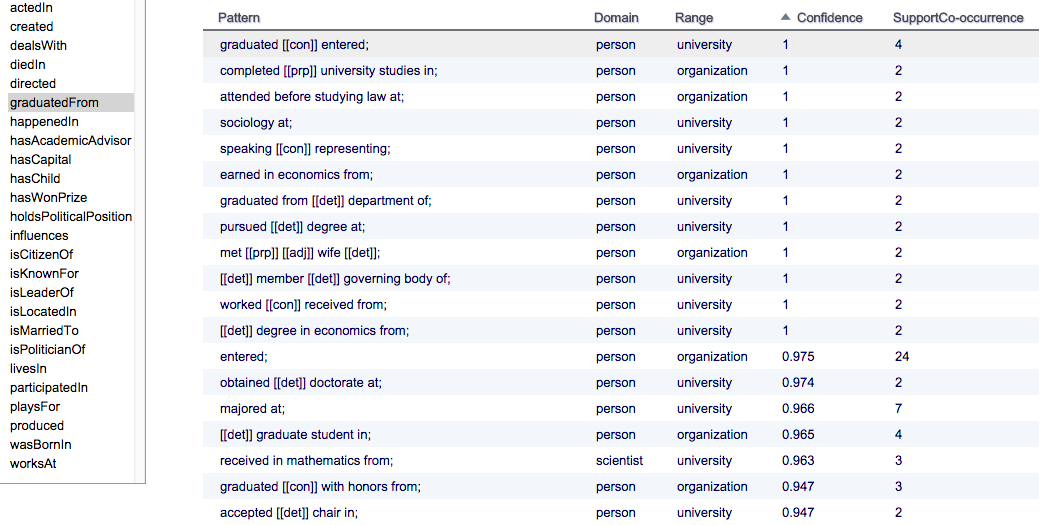
\includegraphics[width=0.8\textwidth]{./images/patty}
  \caption[An example of patterns extracted from PATTY.]{An example of patterns extracted from PATTY for the \emph{graduatedFrom} relation.}
  \label{fig:patty_examples}
\end{figure}

PROSPERA's main technique is that not only it obtain facts based on a small set of initial seed patterns, but also obtain new candidate patterns that can be extrapolated from the corpus based on the mined known facts. Once the process of obtaining new candidate patterns finishes, these are evaluated and then added to the the existing pattern repository for re-use. The whole process then iterates again finding even more facts from these new patterns, and new candidate patterns \cite{Nakashole:2011:SKH:1935826.1935869}. Moreover, another interesting characteristic of the PROSPERA's approach is the care in Entity Disambiguation. For an example, given that in a text it finds a name, such as \emph{\enquote{Captain James Cook}}. It then uses a knowledge base such as YAGO \cite{Suchanek2007} to compare this with existing known entities, using techniques such as N-gram comparison \cite{Nakashole:2011:SKH:1935826.1935869}. With such effort, PROSPERA is able to know that \emph{Captain James Cook} and \emph{James Cook} are actually the same entity with a certain confidence, and thus don't differentiate these and assigns \emph{\enquote{Captain James Cook}} as a representation of the canonical unambiguous entity \emph{\enquote{James Cook}}. This helps in several ways, such as: it can then know other information about this entity, such as the fact that it is of the class \emph{PERSON}; and it can also facilitate future queries in this knowledge base, centralizing the new information found about this existing entity.

Another tool in the Stanford CoreNLP package, the Relation Extractor \cite{Surdeanu:2011:CIE:2021153.2021155} is a classifier to predict relations in sentences. This program has a model that extracts binary relations between entity mentions in the same sentence. The output is normally in the XML \cite{xml} format and denotes the tokens of each sentence, the possible relations, and the confidence level of these relations. The XML demonstrated in Figure \ref{fig:xml_output1} depicts a guess that 2 words in the sentence \emph{\enquote{..., including approaches that use parallel computation [1, 2, 6, 13, 24].}} have the \emph{Uses} relation with a confidence above 70\%. The classifier in this case also indicates that one of the entities is of the class \emph{CONCEPT}.

\begin{figure}[!htbp]
  \centering
    \lstset{
    language=xml,
    tabsize=3,
    %frame=lines,
    %caption=Test,
    %label=code:sample,
    %frame=shadowbox,
    rulesepcolor=\color{blue},
    xleftmargin=20pt,
    framexleftmargin=15pt,
    keywordstyle=\color{blue}\bf,
    commentstyle=\color{OliveGreen},
    stringstyle=\color{red},
    numbers=left,
    numberstyle=\tiny,
    numbersep=5pt,
    breaklines=true,
    showstringspaces=false,
    basicstyle=\footnotesize,
    emph={relation,arguments,entity,span,probabilities,probability,label,value},emphstyle={\color{blue}}
    }
    \lstinputlisting{images/relations.xml}
  \caption[An example of relation extracted with the Stanford Relation Extractor.]{An example of relation extracted with the Stanford Relation Extractor that demonstrated the \emph{\enquote{Uses}} relation.}
  \label{fig:xml_output1}
\end{figure}

As part of its training, annotated relation mentions are used as an input together with the text it belongs to, and the annotation becomes a positive example for the corresponding label, while all the other possible combinations between entity mentions in the same sentence become negative examples. The feature set models the relation between the arguments by using the distance between the relation arguments, the syntactic path between the two arguments, using both constituency and dependency representations.

Note how at this point it's important to no note the notion of a \emph{pipeline} of natural language processing tasks. Stanford's CoreNLP is able to, by itself, perform all the steps needed to produce such relation extraction output from the raw text input. The steps of this pipeline are executed in a certain order, as they depend on the previous step (e.g.: POS tagging is needed for Dependency Parsing). In this case, the process was:

\begin{enumerate}
  \item Tokenize;
  \item Sentence Splitter;
  \item Part-of-Speech tagging;
  \item Lemmatization;
  \item Constituency parsing;
  \item Dependency Parsing;
  \item Named Entity Recognition;
  \item and finally, Relation Extraction.
\end{enumerate}

The Stanford Relation Extractor comes with a model that was trained to extract the following relations: \emph{Live\_In}, \emph{Located\_In}, \emph{OrgBased\_In}, \emph{Work\_For} - and the following classes: \emph{PERSON}, \emph{ORGANIZATION}, \emph{LOCATION}. There are big challenges if one attempts to train the model for any relation outside of these, mainly in obtaining or generating annotated data to train the classifier as to generate a useful model. There are attempts in which relation extraction is not based on annotated data, but on linguistic characteristics of the text itself, such as its semantics. These tools are normally called Open Relation Extractors and will be further described in Section \ref{section:related}.


%
%
% KNOWLEDGE GRAPHS
%
%


\section{Knowledge Graphs}

Knowledge Graphs contain a valuable of information in a structured format, traditionally originally mined from table-like structures form places like Wikipedia \cite{wiki} tables \cite{dbpedia-swj}, or from processes like Information Extraction as described in the previous section. It can be used for a diverse range of applications, such as helping other systems reason about quality of harvested facts \cite{Suchanek2007}, provide table-like facts about an entity \cite{google}, and question-answering systems \cite{hixon-clark-hajishirzi-2015}. Moreover, recent years have witnessed a surge in large scale knowledge graphs, such as DBpedia \cite{dbpedia-swj}, Freebase \cite{Bollacker2008}, Google’s Knowledge Graph \cite{google}, and YAGO \cite{Suchanek2007}.

\begin{figure}[!htbp]
  \centering
    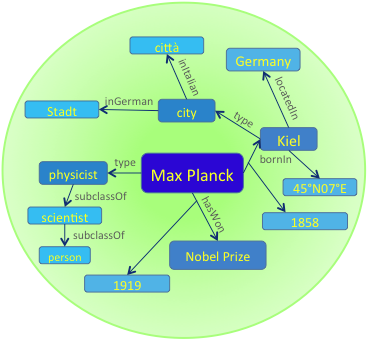
\includegraphics[width=0.6\textwidth]{./images/yago_graph}
  \caption[An example of knowledge graph plotted with vertices and edges.]{An example of knowledge graph from \cite{Suchanek2007} plotted with vertices and edges.}
  \label{fig:yago_knowledge_graph}
\end{figure}

The Knowledge Graph name follows from the data structure that is created from the facts in its final form, a graph with nodes representing entities and edges representing various relations between entities. In Figure \ref{fig:yago_knowledge_graph}, it is possible to observe an example plotted in this form. The list of possible entities classes, and allowable relations between entities is known as a schema. The schema represented in Figure \ref{fig:yago_knowledge_graph} is detailed in Table \ref{tab:max_planck}; one can observe that, as an example, \emph{\enquote{Max Planck}} is an entity of the type \emph{physicist}.

\begin{table}[!htbp]
  \centering
  \RaggedRight
    \texttt{type(A, D) :- type(A, B), subclassOf(B, C), subclassOf(C, D)} \\
  \caption[An example of entailment.]{This entailment example allows one to assert that \texttt{type(Max Planck, person)} is also true, based on the fact tuples presented in Table \ref{tab:max_planck}.}
  \label{tab:entailment_example_max}
\end{table}

\begin{figure}[!htbp]
  \centering
    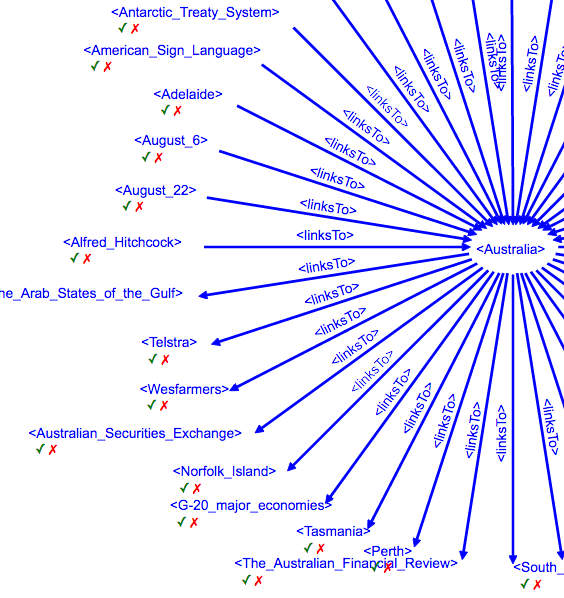
\includegraphics[width=0.6\textwidth]{./images/yago}
  \caption[An example of patterns existants in YAGO.]{An example of patterns existants in YAGO.}
  \label{fig:yago_examples}
\end{figure}

Moreover, based on the facts presented, entailments can be made and one trivial example is denoted in Table \ref{tab:entailment_example_max}. More complex examples of possible reasoning can be seen in \cite{Surdeanu:2011:CIE:2021153.2021155}. This is equivalent to traversing the graph from a node that represents a more specific information, to a node that represents a more general information - e.g.: another possible child node of \emph{\enquote{scientist}} could be the type \emph{\enquote{biologist}}.

\begin{table}[!htbp]
  \centering
  \RaggedRight
    \texttt{type(Max Planck, physicist)} \\
    \texttt{subclassOf(physicist, scientist)} \\
    \texttt{subclassOf(scientist, person)} \\
    \texttt{bornIn(Max Planck, Kiel, 1858)} \\
    \texttt{type(Kiel, city)} \\
    \texttt{locatedIn(Kiel, Germany)} \\
    \texttt{hasWon(Max Planck, Nobel Prize, 1919)} \\
  \caption[Some facts regarding Max Planck.]{Some facts regarding Max Planck, also depicted in Figure \ref{fig:yago_knowledge_graph}.}
  \label{tab:max_planck}
\end{table}

This example denotes a classical domain, more precisely important persons, companies, locations, and the relations between them, in which Information Extraction (IE) tools have been very successful on.

As mentioned previously, YAGO \cite{Suchanek2007} is a prominent Knowledge Graph database, and possesses several advanced characteristics. Every relation in its database is annotated with its confidence value. See the example of the resulting graph in Figure \ref{fig:yago_examples}. Moreover, YAGO combines the provided taxonomy with WordNet \cite{Miller:1995:WLD:219717.219748} and with the Wikipedia category system \cite{wiki}, assigning the entities to more than 350,000 classes. This allow for very powerful querying. Finally, it attaches a temporal and a spacial dimension to many of its facts and entities, being then capable to answer questions such as \emph{when} and \emph{where} such event took place.

WordNet is a semantically-oriented dictionary of English, similar to a traditional thesaurus but with a richer structure \cite{BirdKleinLoper09}. More specifically, it provides relations to synonyms, hypernyms and hyponyms, among others.


%
%
% CHALLENGES AND RELATED WORK
%
%


\chapter{Analysis and Related Work}

This work intends to deliver a tool or a process in which one can extract information from academic text, more specifically Computer Science papers form the Database and Data Mining topics. The intention is to obtain entities, and relations between these entities. The motivation is that, with such tool, one could for an example:
\begin{itemize}
	\item Historically research algorithms that were mostly used during a certain time period;
	\item Find which algorithms are used to resolve, or related to, a certain problem;
	\item Find techniques that improve a certain algorithm problem, among others.
\end{itemize}

\section{Analysis of Academic Text}

The corpus of text used was generated utilising papers published from the following conferences during various years: ACL \cite{acl}, EMNLP \cite{emnlp}, ICDE \cite{icde}, SIGMOD \cite{sigmod}, VLDB \cite{vldb}. More specifically, the section of \emph{Related Work of} these papers were the ones used to build the corpus. This was done due to the characteristics and patterns of this section compared to the rest of the paper. After careful reading, we observed that the \emph{Related Work} section generally contains objective comparisons between other algorithms or softwares in contrast with more opaque or abstract explanations form other parts of the paper. This would mean that this section was a good candidate to start the analysis from. Note the following examples of sentences from the \emph{Related Work} section of papers from the corpus:
\begin{enumerate}
	\item \emph{\enquote{Bergsma et al (2013) show that large-scale clustering of user names improves gender, ethnicity and location classification on Twitter.}}
	\item \emph{\enquote{N-Best ROVER (Stolcke et al, 2000) improves the original method by combining multiple alternatives from each combined system.}}
	\item \emph{\enquote{By partitioning the velocity space, the Bdual -tree improves the query performance of the B x -tree.}}
\end{enumerate}

Entities from academic text in this setting are not as straightforward to define as in, for an example, business news, or criminal news. Observe the following sentence:
\begin{itemize}
	\item \emph{\enquote{Japan's Toshiba Corp said it had nominated Satoshi Tsunakawa, a former head of its medical equipment division, to be its next chief executive officer.}}
\end{itemize}

\begin{table}[!htbp]
  \centering
    \begin{tabular}{ll}
      \textbf{Text}             & \textbf{Entity Type} \\
      Japan                     & LOCATION            \\
      Toshiba Corp              & ORGANIZATION          \\
      Satoshi Tsunakawa         & PERSON           
    \end{tabular}
  \caption[NER from the business news example.]{Examples of Named Entity Recognition (NER) from the business news text example.}
  \label{tab:entities_from_business_text}
\end{table}

From the news text example above, Table \ref{tab:entities_from_business_text} lists the entities that are clearly notes in the text. One can observe a very strong feature which is the common capitalization of the first letter of each of these entities. Another characteristic is how entities from this news text example are \emph{global} or \emph{unconditional}: \emph{\enquote{Japan}} is a location regardless of any condition or any context in this document. Another observation is that, referring to the Stanford's Relation Extraction default relations, \emph{\enquote{Toshiba Corp}} is an organisation \emph{Located\_In} \emph{\enquote{Japan}} regardless of other context in this document. This contrasts with concepts and their relations observed in academic papers, thus that while \emph{\enquote{large-scale clustering}} has the \emph{Improves} with \emph{\enquote{gender classification}} in the context of the paper where this data is presented, it might not be true in all cases.

\begin{table}[!htbp]
  \centering
    \begin{tabular}{ll}
      \textbf{Text}             & \textbf{Entity Type} \\
      Bergsma et al (2013)      & AUTHOR          \\
      large-scale clustering    & CONCEPT         \\
      gender classification     & CONCEPT         \\
      ethnicity classification  & CONCEPT         \\
      location classification   & CONCEPT         \\
    \end{tabular}
  \caption[NER from the academic text example.]{Examples of Named Entity Recognition (NER) from the academic text example.}
  \label{tab:entities_from_academic_text}
\end{table}

Moreover, the entities in Table \ref{tab:entities_from_academic_text} are harder to classify in universally agreed classes. For an example, \emph{\enquote{gender classification}} can be considered an action, or a task, or an algorithm. More generally, one can simply classify these as concepts.

\begin{table}[!htbp]
  \centering
  \RaggedRight
    \texttt{IsA(Concept,Concept)} \\
    \texttt{SimilarTo(Concept,Concept)} \\
    \texttt{Improves(Concept,Concept)} \\
    \texttt{Employs(Concept,Concept)} \\
    \texttt{Uses(Concept,Concept)} \\
    \texttt{Supports(Concept,Concept)} \\
    \texttt{Proposes(Author,ComplexConcept)} \\
    \texttt{Introduces(Author,ComplexConcept)} \\
  \caption[Some observed and possible relations between concepts.]{Some observed and possible relations between concepts.}
  \label{tab:possible_academic_relations}
\end{table}

Other possible relations from the Stanford Relation Extractor standard relations that are applicable to the above news text example are: \emph{OrgBased\_In} (again for \emph{\enquote{Toshiba Corp}} and \emph{\enquote{Japan}}) and \emph{Work\_For} regarding its newly placed chief executive officer. Again, contrasting with the academic text, one might consider relations such as the one possibles between concepts as denoted in Table \ref{tab:possible_academic_relations}. In fact, by analysing the corpus for the top 50 words in the singular third-person form, such as \emph{\enquote{improves}} or \emph{\enquote{employs}}, one can have an idea of the possible relations that can be extracted. This process is illustrated in Figure \ref{fig:words_most_used_all}. The same data is illustrated in Figure \ref{fig:words_most_use_no_top2}, but with the top two words removed (\emph{\enquote{is}} and \emph{\enquote{has}}).

\begin{figure}[!htbp]
  \centering
    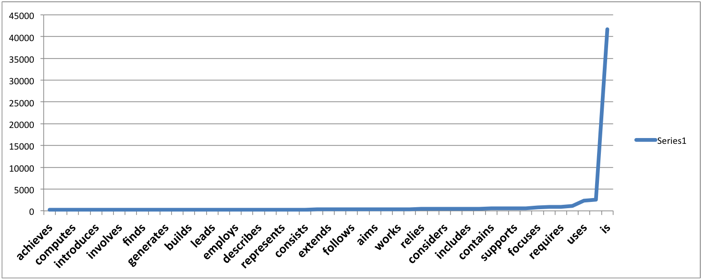
\includegraphics[width=1.0\textwidth]{./images/words_most_used_all}
  \caption[Samples of the most common words in the singular third-person form.]{Samples of the most common words in the singular third-person form. The \emph{y} axis represents the number of times the word in the \emph{x} axis appeared in the text.}
  \label{fig:words_most_used_all}
\end{figure}

\begin{figure}[!htbp]
  \centering
    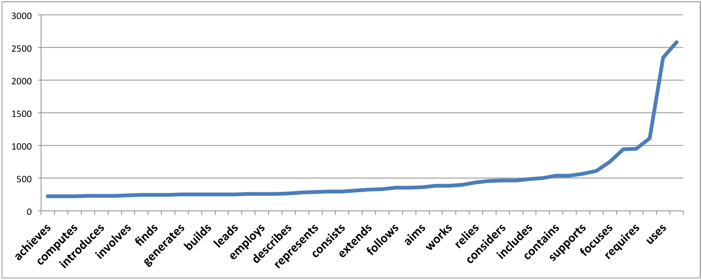
\includegraphics[width=1.0\textwidth]{./images/words_most_use_no_top2}
  \caption[Samples of the most common words in the singular third-person form, after removing the top 2 words.]{Samples of the most common words in the singular third-person form, after removing the top 2 words (\emph{\enquote{is}} and \emph{\enquote{has}}). The \emph{y} axis represents the number of times the word in the \emph{x} axis appeared in the text.}
  \label{fig:words_most_use_no_top2}
\end{figure}

One of the initial attempts to explore how to extract information from the generated corpus was to use the Stanford Named Entity Recognizer (NER) to recognize the concepts discussed so far in the academic text. To do so, a small set of around 20 papers' \emph{Related Work} section was annotated for the concepts contained in them using Brat \cite{Stenetorp:2012:BWT:2380921.2380942}. An example of this annotated data can be seen in Figure \ref{fig:brat_img}.

The annotated data is then transformed form Brat's standoff format \cite{Stenetorp:2012:BWT:2380921.2380942} into a Table Separated Value (TSV) format, using a custom script, based on customised version of from standoff2conll \cite{standoff2conll}, renamed standoff2others. The output is similar to the one showed in Table \ref{tab:james_cook_iob}, but its simplified version without the \emph{B-} and \emph{I-} prefixes.

The model was trained mostly with the recommended settings and features, such as the word itself, its class, surrounding words and word shapes. When applying this trained NER model (Figure \ref{fig:stanford_ner_usage}), we observed that the success was moderated, as it was, at times, able to detect clearly delineated concepts by its shape (.e.g: capital words), but for non-capitalized words it appeared as it would only recognize the concepts if its words were present in the training set.

\begin{figure}[!htbp]
  \centering
    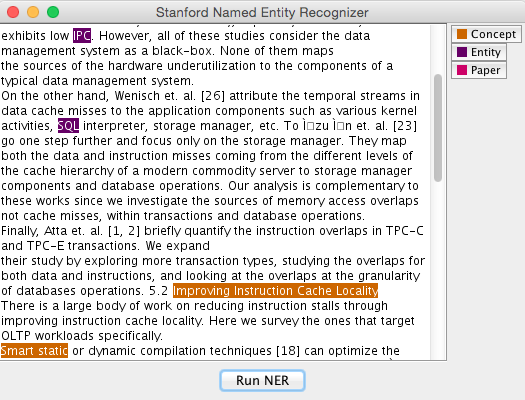
\includegraphics[width=0.9\textwidth]{./images/stanford_ner}
  \caption[The Stanford NER GUI (Graphic User Interface) using our trained model.]{The Stanford NER GUI (Graphic User Interface) using our trained model.}
  \label{fig:stanford_ner_usage}
\end{figure}

In this image, please observer the attempt of differentiate entities such as \emph{CONCEPT} and \emph{ENTITY}. We also annotated references to other papers using the \emph{PAPER} entity, in general they appears as numbers between square brackets. Initially, we attempted to annotated using a hierarchy where entities were very specific proper nouns, while concepts had a more loose definition, and would likely be more general concepts. During the process, however, this type of annotation also proved to be difficult as it would require domain-specific knowledge of very deep database discussions in order to differentiate concepts by these two classes, and could still sometimes generate debates.

As an attempt of further improve the quality of the NER model, we made use of a gazetteer. As part of this research, the Microsoft Academic Graph \cite{microsoft-academic-data} was found to contain a very relevant list of \emph{keywords} and \emph{fields of study} available for download and academic use. Another custom script was developed to transform the data from the format provided by Microsoft into the input format accepted by Stanford's NER shown in Table \ref{tab:concept_list_from_gazetteer}. The Stanford NER utilises the gazetteer input in both ways: matching the concepts token by token in their entirety, or in a \enquote{sloppy} manner accepting a positive match even if only one of the tokens in the gazetteer entry had a match \cite{Finkel:2005:INI:1219840.1219885}. In both cases, however, the gazetteer is treated simply as another feature and does not guarantee that if the entries are found in the text they would be marked as an entity \cite{Finkel:2005:INI:1219840.1219885}. The gazetteer format has its first token denoting the type of the entry, all of the type \emph{CONCEPT} in this case, with the following words denoting the gazetteer entry itself, space separated. We did not observed improvement with this addition.

\begin{table}[!htbp]
  \centering
    \begin{tabular}{l}
CONCEPT SMOOTHSORT \\
CONCEPT CUSTOMISED APPLICATIONS FOR MOBILE NETWORKS \\
CONCEPT XML DOCUMENTS \\
CONCEPT JOSEPHUS PROBLEM \\
CONCEPT RECOGNIZABLE 
    \end{tabular}
  \caption[Format in which Stanford's NER supports a gazetteer input.]{Format in which Stanford's NER supports a gazetteer input.}
  \label{tab:concept_list_from_gazetteer}
\end{table}

The next step was to attempt to use the Stanford Relation Extractor (RE). The same small annotated sample by us in Brat would also contain the following relations: \emph{Improves}, \emph{Worsen}, \emph{IsA}, \emph{Uses}. The standoff2others custom library was then improved to be able to generate the more complex CoNLL format, accepted as an input for training of the Stanford's RE, denoted in Table \ref{tab:format_for_relation_extractor_input} \cite{Surdeanu:2011:CIE:2021153.2021155}. Also, the Java parser code from the Relation Extractor had to be changed in a few places to accept custom labels (classes) for NER.

\begin{table}[!htbp]
  \centering
    \begin{tabular}{lllllllll}
2 &	Concept &	0 &	O &	NNP/NNS &	LSH/functions &	O &	O &	O \\
2 &	O &	1 &	O &	VBP &	are & 	O &	O &	O \\
2 &	O &	2 &	O &	NFP &	fi &	O &	O &	O \\
2 &	O &	3 &	O &	RB &	 rst &	O &	O &	O \\
2 &	O &	4 &	O &	VBN &	introduced &	O &	O &	O \\
2 &	O &	5 &	O &	IN &	for &	O &	O &	O \\
2 &	O &	6 &	O &	NN &	use &	O &	O &	O \\
2 &	O &	7 &	O &	IN &	in &	O &	O &	O \\
2 &	Concept &	8 &	O &	NNP/NN &	Hamming/space &	O &	O &	O \\
2 &	O &	9 &	O &	IN &	by &	O &	O &	O \\
2 &	O &	10 &	O &	NNP &	Indyk &	O &	O &	O \\
2 &	O &	11 &	 O &	CC &	and &	O &	O &	O \\
2 &	O &	12 &	O &	NNP &	Motwani &	O &	O &	O \\
2 &	O &	13 &	O &	-LRB- &	[ &	O &	O &	O \\
2 &	O &	14 &	O &	CD &	7 &	O &	O &	O \\
2 &	O &	15 &	O &	-RRB- &	] &	O &	O &	O \\
2 &	O &	16 &	O &	. &	. &	O &	O &	O \\
 & & & & & & & & \\
0 & 8 & Uses & & & & & & \\
    \end{tabular}
  \caption[Format in which Stanford's Relation Extractor accepts its training input.]{Format in which Stanford's Relation Extractor accepts its training input.}
  \label{tab:format_for_relation_extractor_input}
\end{table}

The important columns of this format are: column 2 which denotes the entity tag, column 3 denotes the token ID in the sentence, column 5 contains its Part-Of-Speech tag, and column 6 which contains the token itself. For this specific process, POS tags were obtained from the Google Syntaxnet Software \cite{google-syntaxnet, DBLP:journals/corr/AndorAWSPGPC16}, which were generated in separated and then joined with the token for the final CoNLL output.

The results from the RE trained model, one of which is depicted in Figure \ref{fig:xml_output1}, were much poorer compared to the NER output, and we failed to find interesting relations with confidences above 50\%. In both cases, after analysing the models we were able to generate using the NER and the Relation Extractor software from Stanford, it was clear that much more annotated data would be needed as to achieve higher quality results.

Please refer to Section \ref{section:tools} for more information on tools mentioned in this section.


%
%
% RELATED WORK
%
%


\section{Open Information Extraction}
\label{section:related}

Since we had no access to annotated data, we turned to a different approach called Open Information Extraction in an attempt for better results. This approach uses linguistic information from the text, among other techniques, as to attempt to extract the relations without the need of a trained model.

\hl{- Attempt of using Stanford OpenIE}

\hl{- Heuristics attempted with OpenIE results}

\hl{To be completed: Querying a corpus? How to check for similar words statistically, etc}

\hl{- Any further results? Review code for other code.}


Other methods for relation extraction such as the ones from papers:

ClausIE: Clause-Based Open Information Extraction

Extreme Extraction: Only One Hour per Relation

IKE - An Interactive Tool for Knowledge Extraction

All tools described in this section are similar in nature to our tool, thus describing the related work.


%
%
% PECULIARITIES OF ACADEMIC TEXT
%
%


\section{Peculiarities with Academic Text}

Problem accross domains, strict language vs. creative language.

Sarcasm.

We are extracting explicit information, and not trying to infer implicit information. That would be a different logical problem that would need to reason about using a database of information to compare what is being learned from the natural text with.

Difficult to manually tag.

Existing tools that are based in models don't come equiped to predict relation in this kind of text. E.g.:

Relations that could be extracted, e.g. defines, don't appear with relevant Entities.

A lot of coreference problems, e.g. "their work". Even when their work is simply a paper reference - with unclear. One could trivially parse the above reference with the actual Entity name of the system or algorithm or technique elabrated in the reference paper as to mine the relations between the proper entities.

Methods:

* Use semi-automatic methods to collect research literature and convert them into plain text with certain markups. 
* Use existing open source solutions to parse the store the input data. 
* Build a pipeline to extract entities and relationship from the input data. 
* Perform entity disambiguation and linking to a reference Knowledge Graph (e.g., Yago2 or DBPedia). 
* Design effective postprocessing methods to improve the quality of the extraction.
* Evaluate the entire extraction system.


%
%
% DEVELOPED WORKFLOW
%
%


\chapter{Developed Workflow}

\hl{The first step to in achieving our goal is obtaining the raw natural language text from papers in the area. Most research products such as thesis, papers, or any other report, are mostly available primarily in the Portable Document Format (PDF) format} \cite{pdf} \hl{- which then needs to then be parsed into a raw text in an automated manner.}


%
%
% USED TOOLS
%
%


\section{Tools}
\label{section:tools}

\subsection{PDF extraction generates noisy output}

\subsection{Programming Languages}

Java

Python

\subsection{Python Modules}

requests

BeautifulSoup4

standoff2conll

corpkit

Tregex

corenlp-xml

\subsection{NLTK}

\subsection{Brat}

\begin{figure}[!htbp]
  \centering
    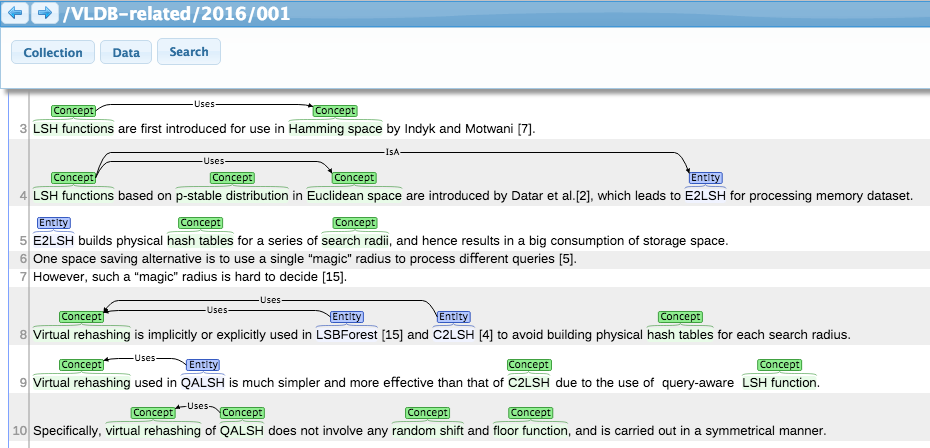
\includegraphics[width=1.0\textwidth]{./images/brat_img}
  \caption[The Brat rapid annotation tool, an online environment for collaborative text annotation.]{The Brat rapid annotation tool, an online environment for collaborative text annotation.}
  \label{fig:brat_img}
\end{figure}


\subsection{Jupyter}

\subsection{Parsey}

\subsection{SpaCy}

\subsection{Stanford CoreNLP}

\subsection{Graphviz}


%
%
% DEVELOPED PROCESS AND PROGRAMS
%
%


\section{Developed process and programs}

verb-centric

----------------------
Attempted to generate a parametrized relation with "options", such as:
http://verbs.colorado.edu/propbank/framesets-english-aliases/improve.html

We might use their results as a reference for our own grouping. 
For more info on these resouces, a quick slides is http://faculty.ist.unomaha.edu/ylierler/teaching/material/sp13/FrameNetPropBankVerbNet.pptx
----------------------

Q-TREE

We use some pair of delimiter (e.g., [, ] as you used) to enclose each subtree. (this is similar to lisp). 

u [ a [ b c d]
     e [f [g h] i]
     k 
   ]

btw, this is very similar to q-tree's syntax: 

http://texdoc.net/texmf-dist/doc/latex/tikz-qtree/tikz-qtree-manual.pdf

----------------------

To some extent, our current approach is similar to that of ClauseIE, but with several key differences:

* We tailor the extraction process for each different verb, as long as there is a sufficiently large corpus to find typical usage of the verbs.

* Instead of heuristically determining whether or which PP-attachment (named 'A' as in SVAA) to be used as object of the verb, we can do it more accurately given the verb and example sentences. It is also desirable for us to look for exceptions proactively, probably by using (enhanced) regexp matching (e.g., 'improve (up)on */VBG ...')

* Also we extract more than binary relation with an optional typeless argument as ClauseIE did. The output is more inline with these semantic functional analysis of verbs (e..g, as in PropBank, etc.).

* I cannot remember clearly, but I don't think ClauseIE tried hard to find the right NP (if existings) as the `subj` or `obj` argument of the verb. This is pretty important for KG (esp. for reasoning) and technically challenging too. But I do expect rules/experience gained in this aspect can be easily transferred to other verbs - that's the meta-rule I mentioned yesterday.


%
%
% RESULTS
%
%


\chapter{Results}

\hl{- Evaluation}

----------------------
"improves" is an intransitive verb, hence there is no dobj. (the last few groups). 
----------------------


%
%
% CONCLUSION AND FUTURE WORK
%
%


\chapter{Conclusion and Future Work}

\hl{- What drives the field forward}d

Furhter ideas:
- Research relations through time. You could have a certain feature.
- Reinforcements made to definitions in other papers.
- Events, such as changes in conclusions - e.g.: this was the better technique, now this other technique is the best.

\backmatter

\printbibliography

\appendix

\end{document}